%\documentclass{article}
%\usepackage{fixltx2e}
%\usepackage{graphicx}
%\usepackage{caption}
%\usepackage{subcaption}
%
%\begin{document}
\subsection*{}
In this section we will describe about our tree construction \emph{US-tree}. We have describe earlier about our batch and window. A batch should be inserted into the tree in it's own window slot. After inserting all batches of to full the window, the window shall be complete and be ready to mine. We said earlier section that our tree will be very compact. For this we have proposed an approach for sharing nodes. For sharing same tree nodes two items with same id and order should not care about own existential probability. If item is already in the tree with same id then two items should share the node. Thus the tree will be very compact. When inserting an item in the tree the \emph{U\textsuperscript{cap}}  of the tree should be updated by adding the prefix value of the node. Thus each batch should be inserted into the tree. The algorithm is given in the algorithm section Algorithm-\ref{algorithm:tree_construction}.
%\documentclass{article}
%\usepackage{graphicx}
%\usepackage{caption}
%\usepackage{subcaption}
%
%\begin{document}
\begin{figure}[!tbp]
  \centering
	\fbox{  
	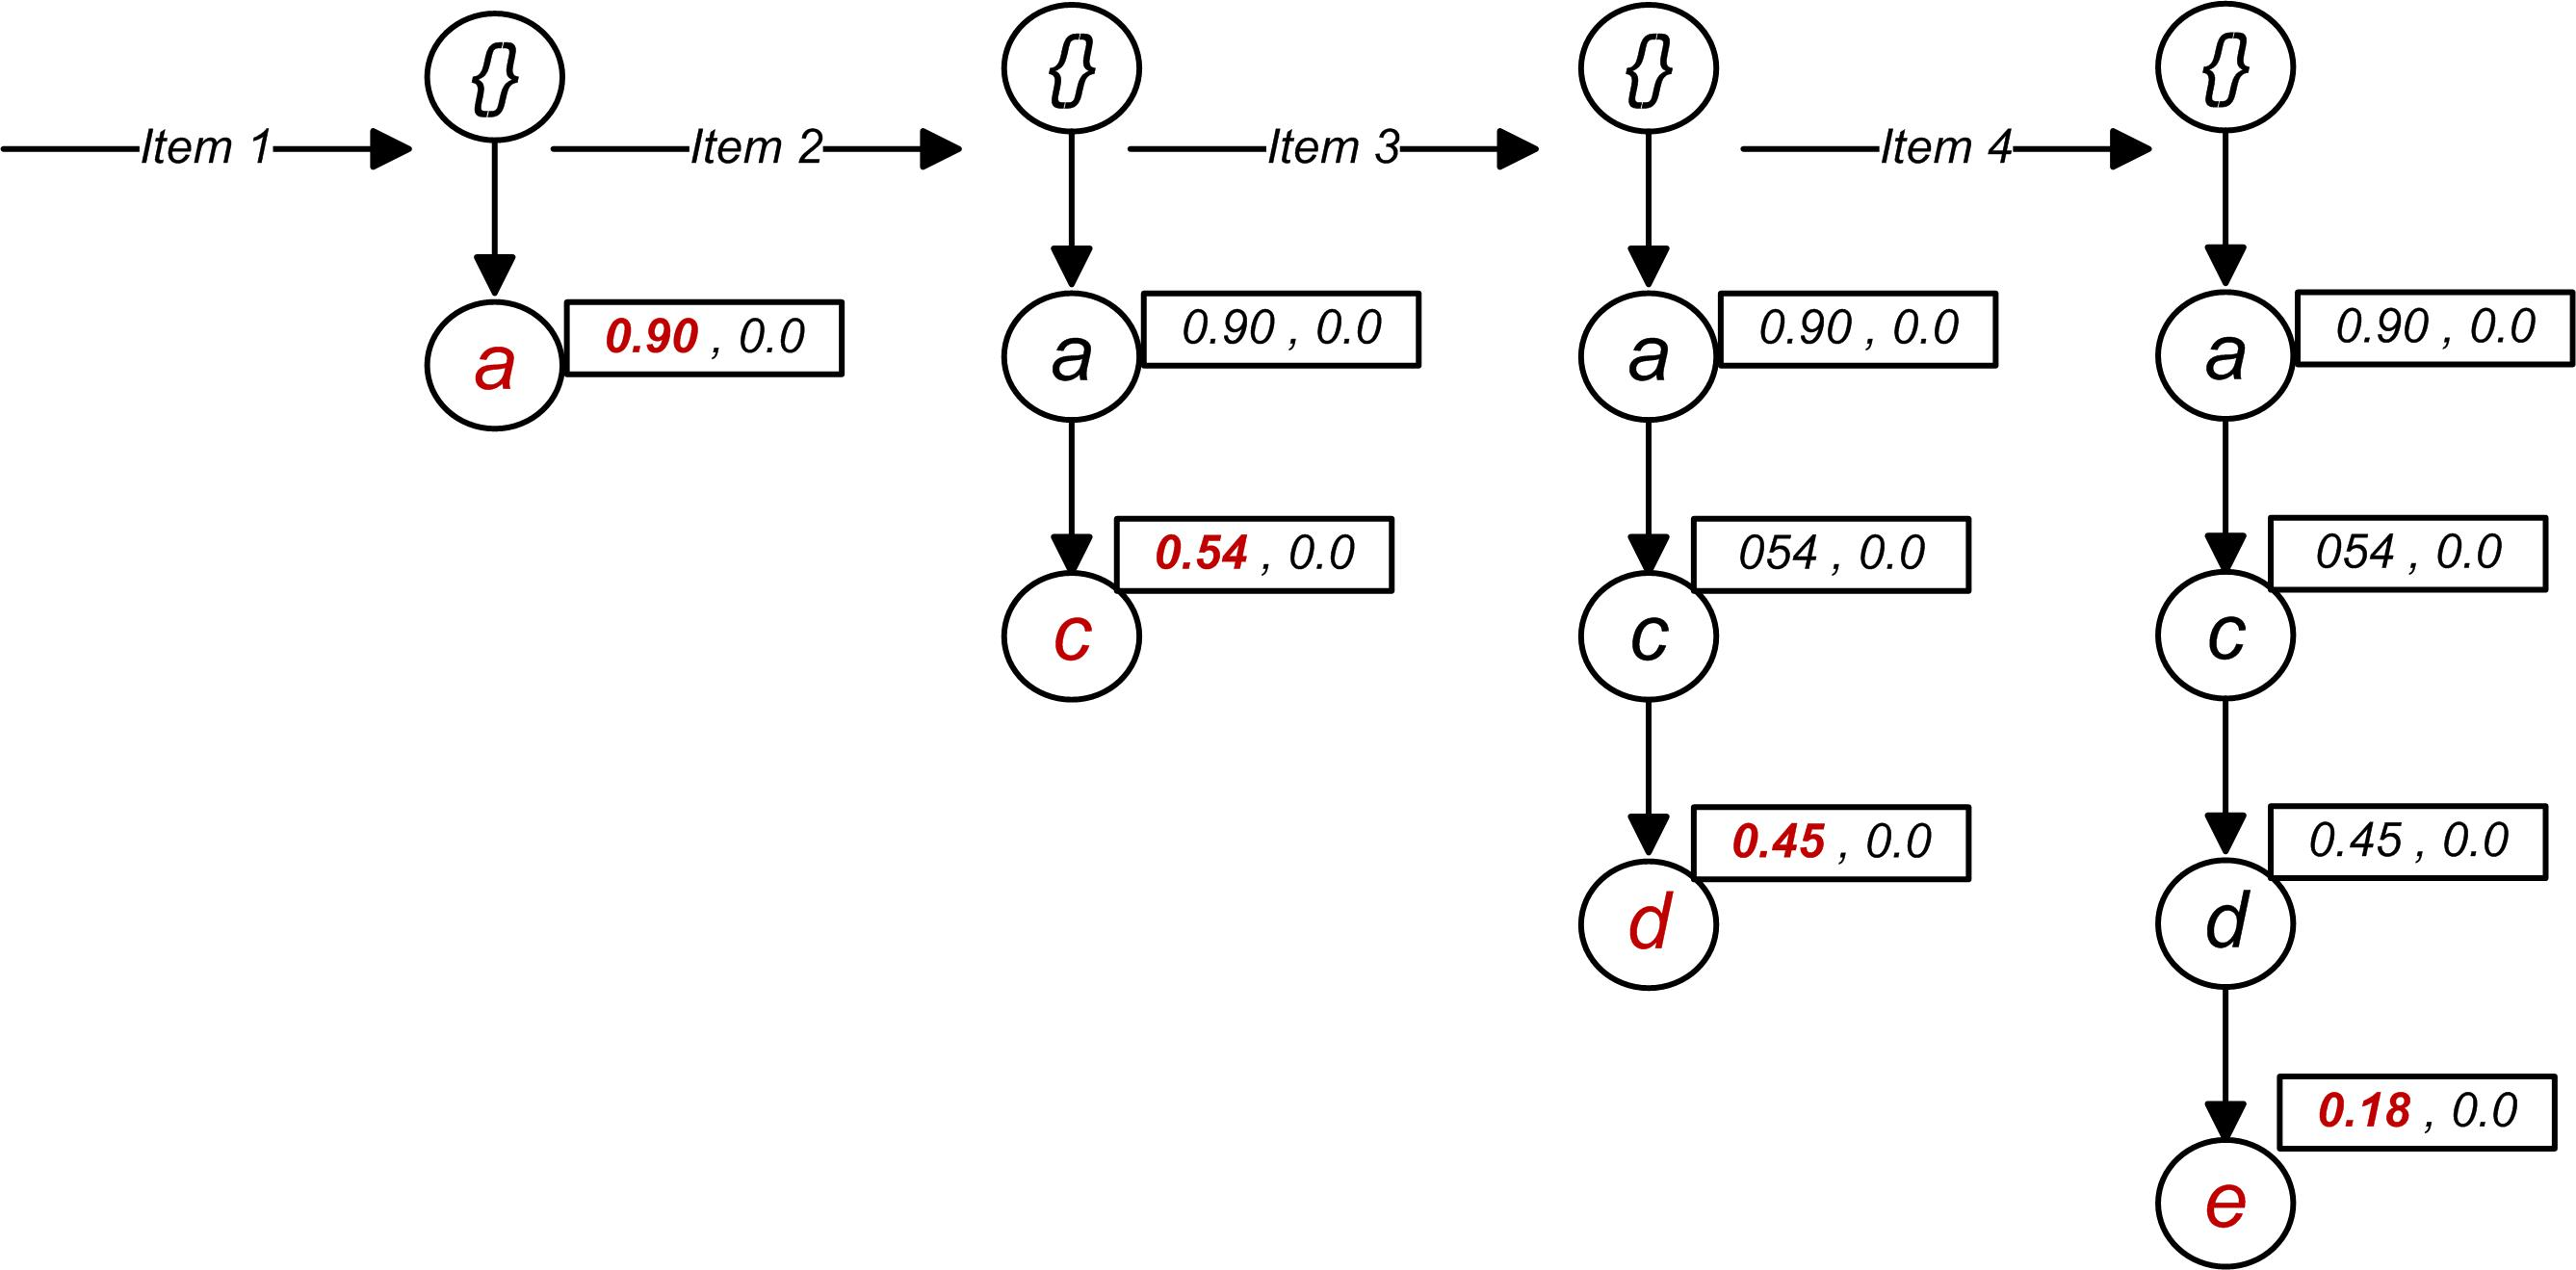
\includegraphics[width=.8\textwidth,height=5cm]{images/sim_01.jpg}  
	}
	\caption{Inserting \emph{T\textsubscript{1}} into \emph{US-tree}}
	\label{figure:t1}
\end{figure}
\begin{frame}

\begin{figure}[!tbp]
  \centering
	\fbox{  
	 	\begin{subfigure}[b]{0.40\textwidth}
	 	\centering
	    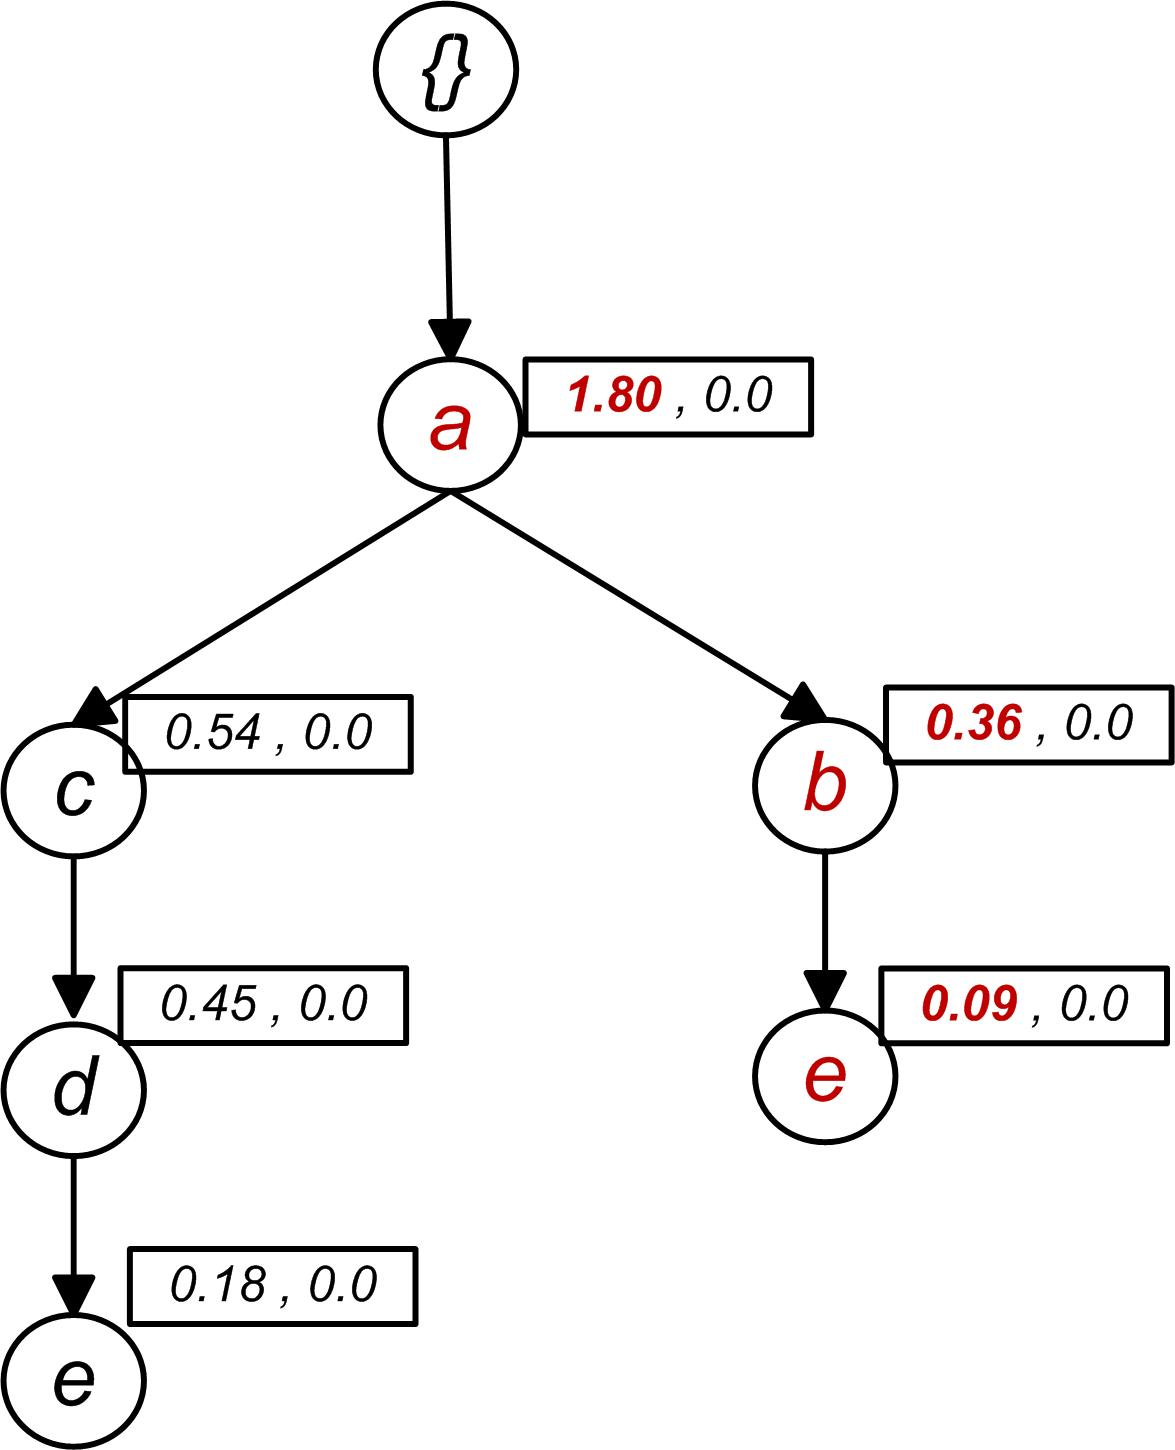
\includegraphics[width=.8\textwidth,height=4cm]{images/sim_02.jpg}
	    \caption{T\textsubscript{2}}
		\end{subfigure}
	  
	 	\begin{subfigure}[b]{0.40\textwidth}
	 	\centering
	    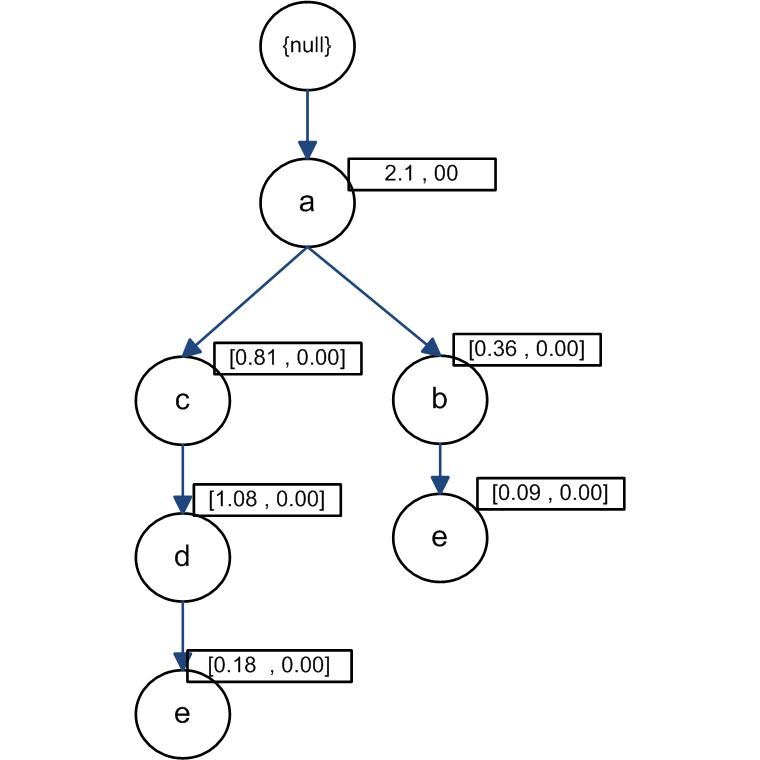
\includegraphics[width=.8\textwidth,height=4cm]{images/sim_03.jpg}
	    \caption{T\textsubscript{3}}
		\end{subfigure}
	}
 \caption{Inserting \emph{T\textsubscript{2}} and \emph{T\textsubscript{3}} in \emph{US-tree}}
 \label{figure:t23}
\end{figure}
\end{frame}
\begin{frame}

\begin{figure}[!tbp]
  \centering
	\fbox{  
	 	\begin{subfigure}[b]{0.22\textwidth}
	 	\centering
	    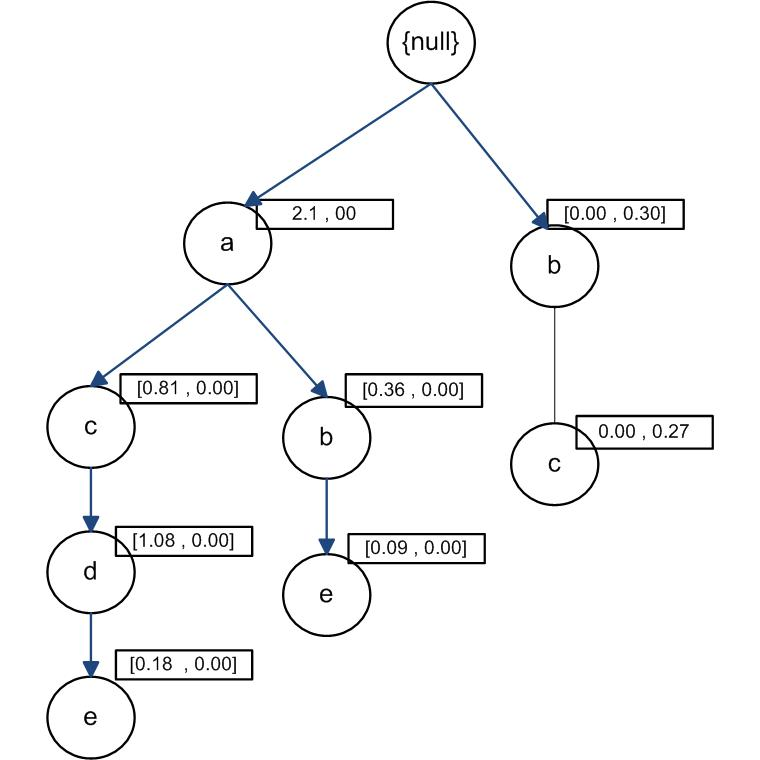
\includegraphics[width=\textwidth,height=4.0cm]{images/sim_04.jpg}
	    \caption{T\textsubscript{4}}
		\end{subfigure}
	 
	 	\begin{subfigure}[b]{0.27\textwidth}
	 	\centering
	    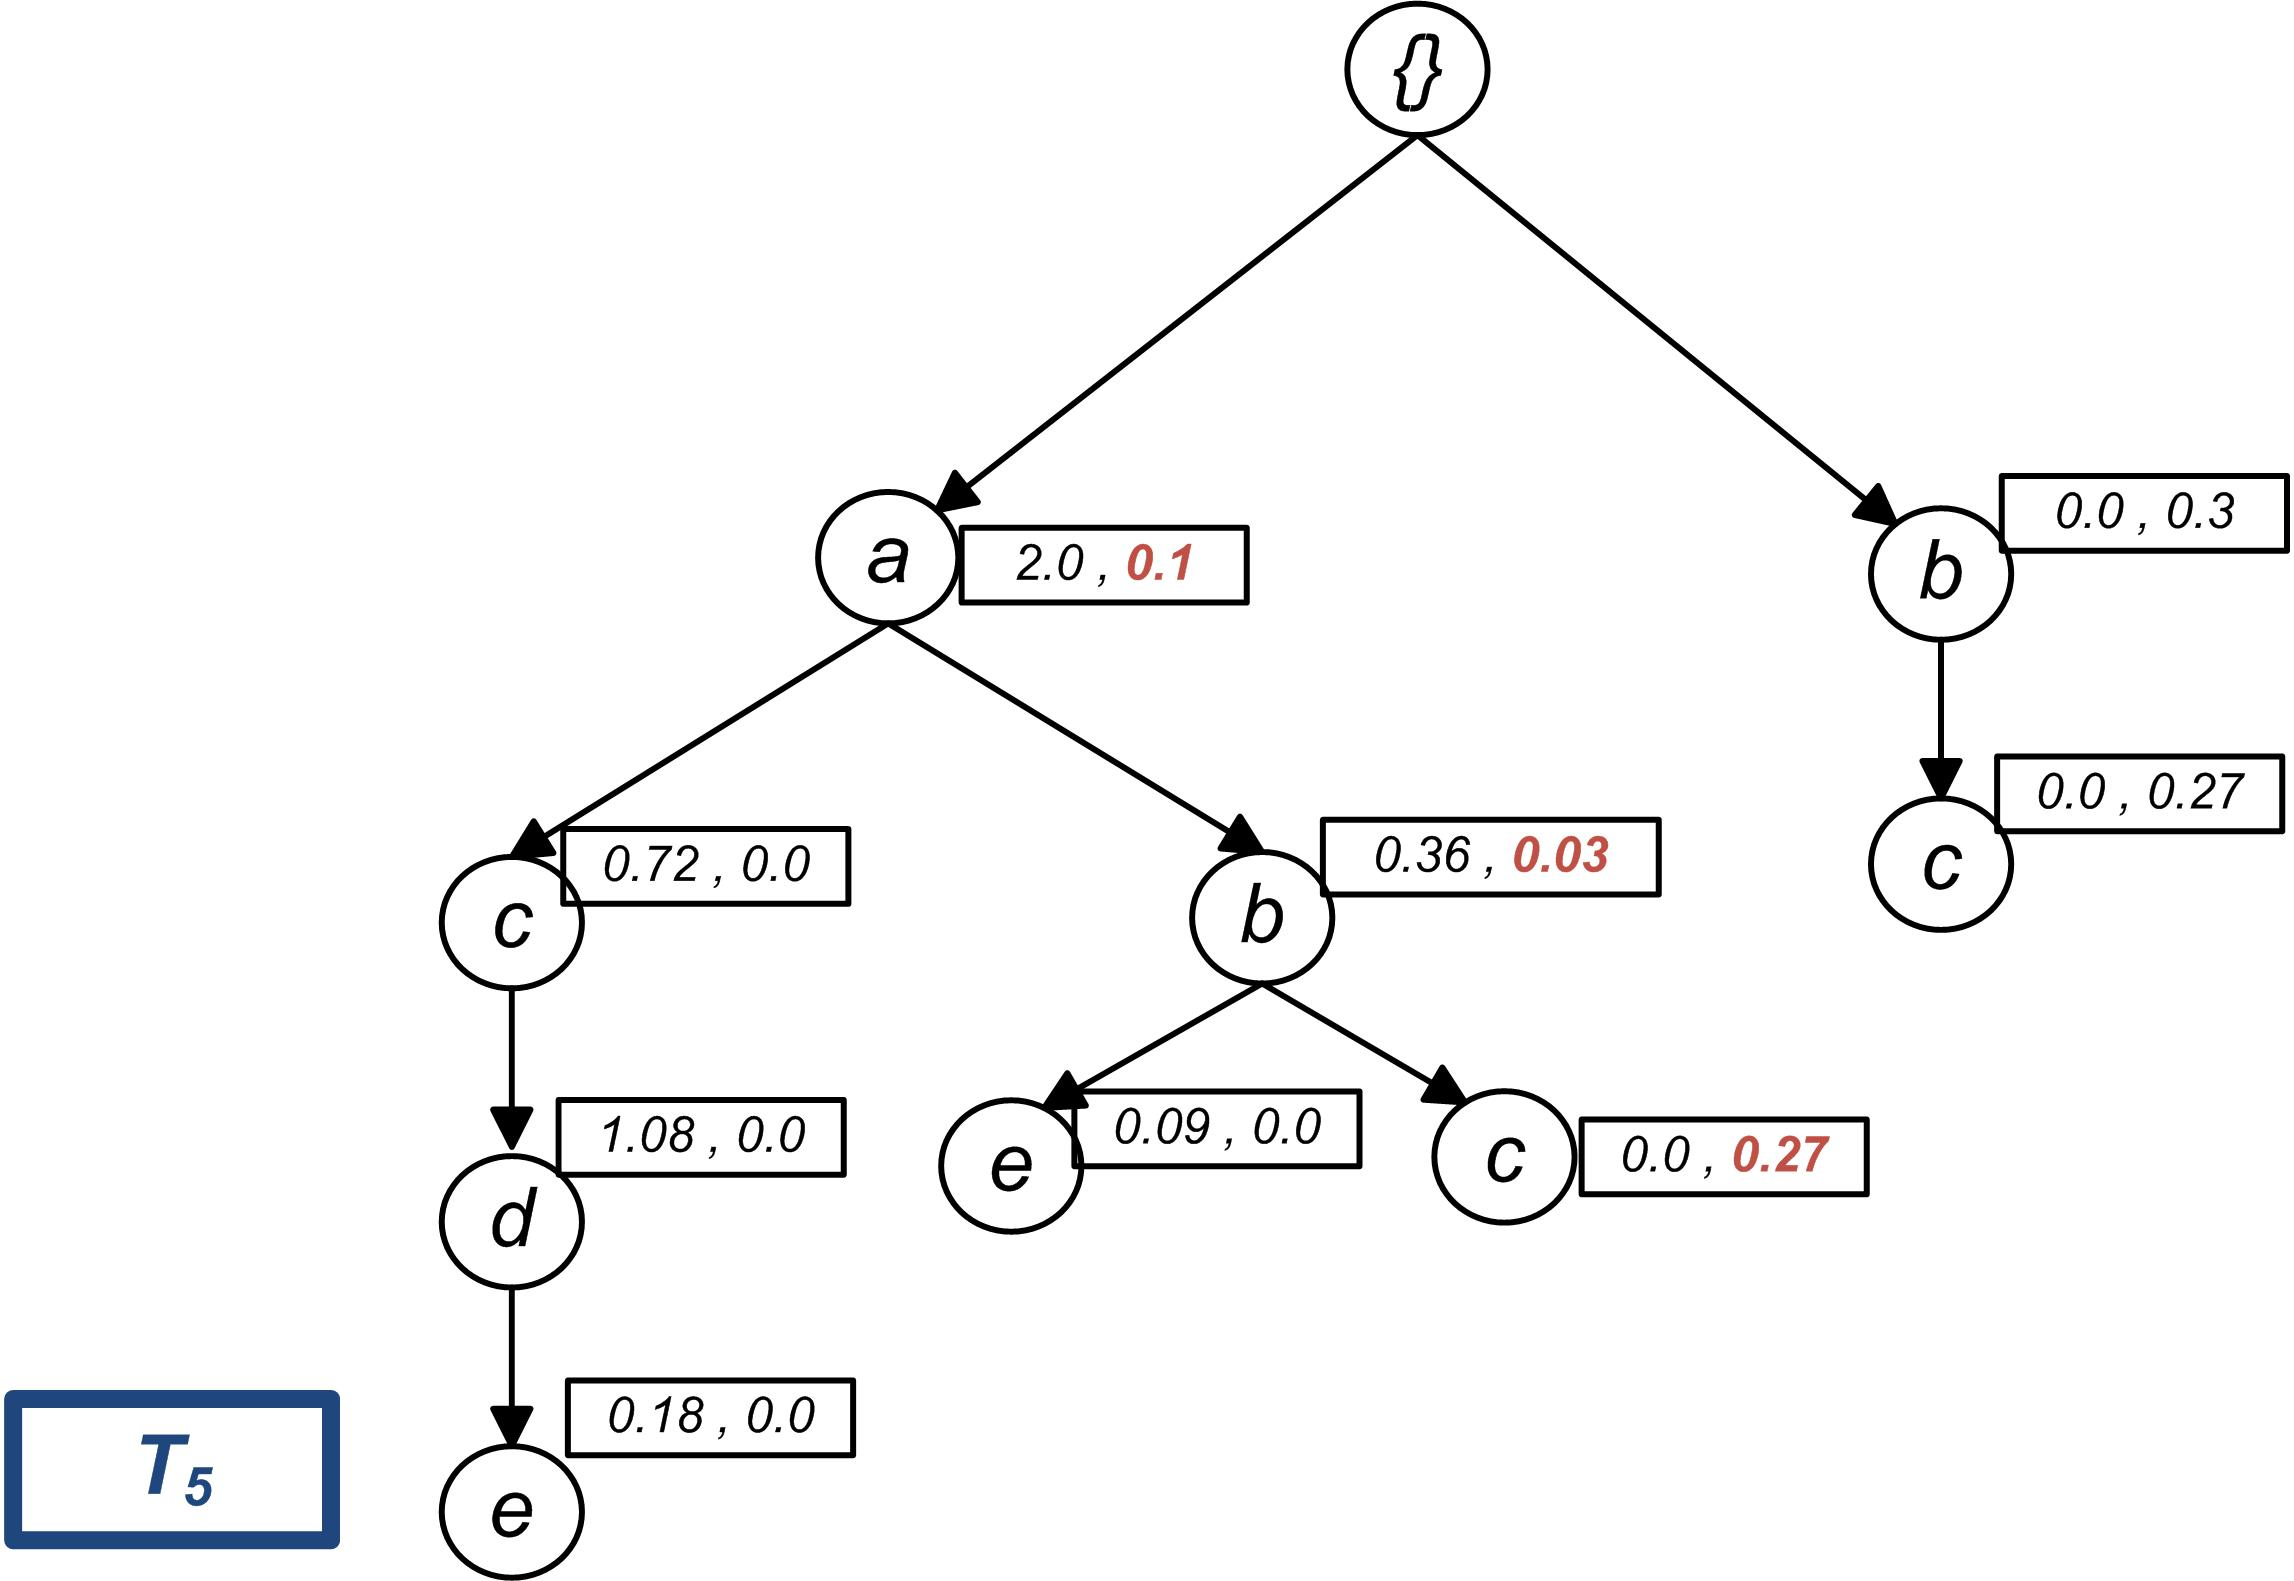
\includegraphics[width=\textwidth,height=4.0cm]{images/sim_05.jpg}
	    \caption{T\textsubscript{5}}
		\end{subfigure}
	  
	 	\begin{subfigure}[b]{0.31\textwidth}
	 	\centering
	    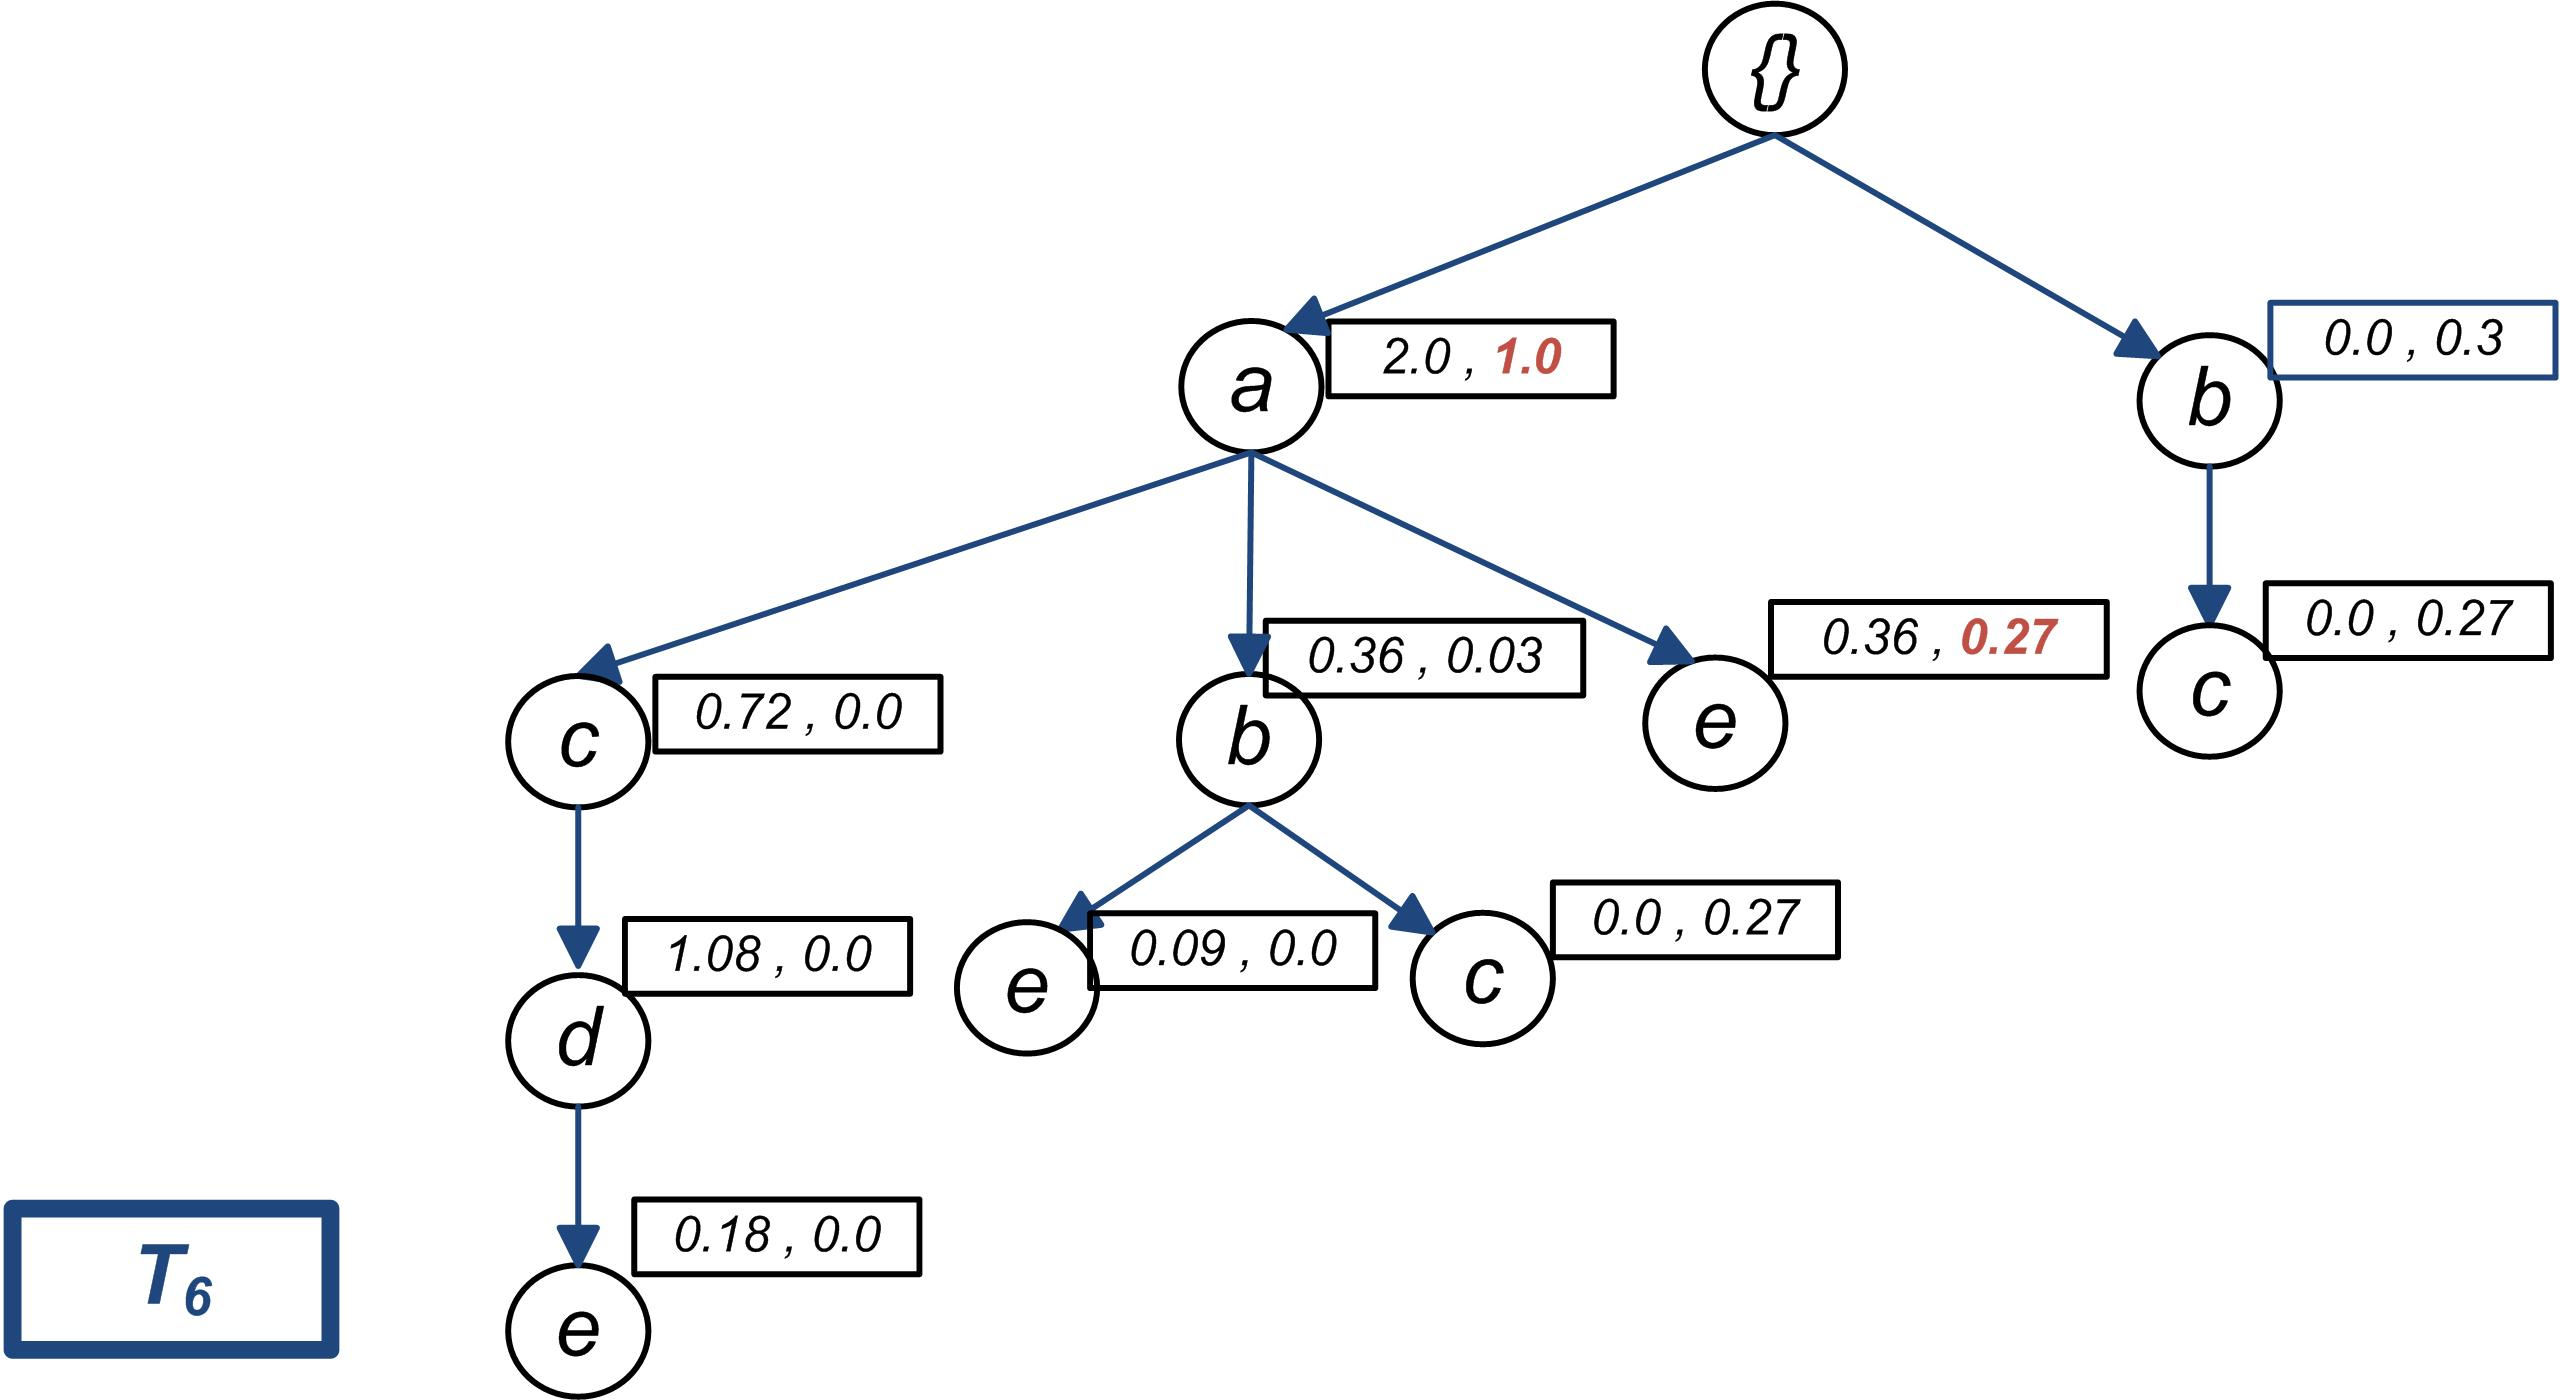
\includegraphics[width=\textwidth,height=3.0cm]{images/sim_06.jpg}
	    \caption{T\textsubscript{6}}
		\end{subfigure}
	}
 \caption{Inserting \emph{T\textsubscript{4}},\emph{T\textsubscript{5}} and \emph{T\textsubscript{6}} in \emph{US-tree}}
 \label{figure:t456}
\end{figure}
\end{frame}
%\end{document}
\subsection*{}
Let construct tree for Table-\ref{table:prefix_assigned}. First we insert \emph{Batch-1 (T\textsubscript{1}, T\textsubscript{2}, T\textsubscript{3})} in the window 1. First when inserting the \emph{T\textsubscript{1} - a(0.9), c(0.54), d(0.45), e(0.18)} we insert item \emph{a(0.9)} as a child of root \emph{\{\}} (Figure-\ref{figure:t1}). Update a's prefix value as $0.9$. Then we add \emph{c(0.54)} as a's child update c's prefix value as $0.54$. Aad \emph{d(0.45)} as c's child update d's prefix value as $0.45$. Add \emph{e(0.18)} as d's child update e's prefix value as $0.18$. Thus \emph{T1} is inserted into the tree (Figure-\ref{figure:t1}). For \emph{T\textsubscript{2} - a(0.9), b(0.36), e(0.09)} first we insert \emph{a(0.9)}. Here we found \emph{a} is already inserted so we just update existing node a's prefix value $0.9 + 0.9 = 1.8$ (Figure-\ref{figure:t23}). Then we insert \emph{b(0.36)}. As \emph{a} has no child \emph{b} we insert a new child b and update it's prefix value $0.36$. Then insert new e(0.09) as the child of \emph{b}. For \emph{T\textsubscript{3} - a(0.2), c(0.18), d(0.63)} we follow the existing path \emph{a(1.8), c(0.54), d(0.45)} and update corresponding prefix value as $1.8 + 0.2 = 2.0$, $0.54 + 0.18 = 0.72$ and $0.45 + 0.63 = 1.08$ (Figure-\ref{figure:t23}). After inserting the This \emph{T\textsubscript{3}} window 1 is completed. Then we will go for inserting next batch \emph{Batch-2 (T\textsubscript{4}, T\textsubscript{5}, T\textsubscript{6})} in the tree. For \emph{Batch-2} we shall put prefix value in the window's newest place. And thus the latest batch becomes the most recent information. For inserting \emph{T\textsubscript{4} - b(0.3), c(0.27)} we insert new node \emph{b} as there is no child b of root node \emph{\{\}}. So we insert \emph{b} as a child of root \emph{\{\}}. update its prefix value as $0.3$. Then insert \emph{c(0.27)} as child of \emph{b} and update prefix value $0.27$. Here as this \emph{T\textsubscript{4}} is inserting in \emph{Batch-4} we update prefix value for recent batch's information. Next we insert \emph{T\textsubscript{5} - a(0.1), b(0.03), c(0.27)}. We merge \emph{a(0.1), b(0.03)} with previous \emph{a, b } nodes and update prefix value $0.1$ and $0.03$ in the second batch's portion and insert new node \emph{b} as a child of \emph{b} and update its prefix value as $0.27$ (Figure-\ref{figure:t456}).
%\documentclass{article}
%\usepackage{graphicx}
%\usepackage{caption}
%\usepackage{subcaption}
%
%\begin{document}
\begin{figure}
  \centering
	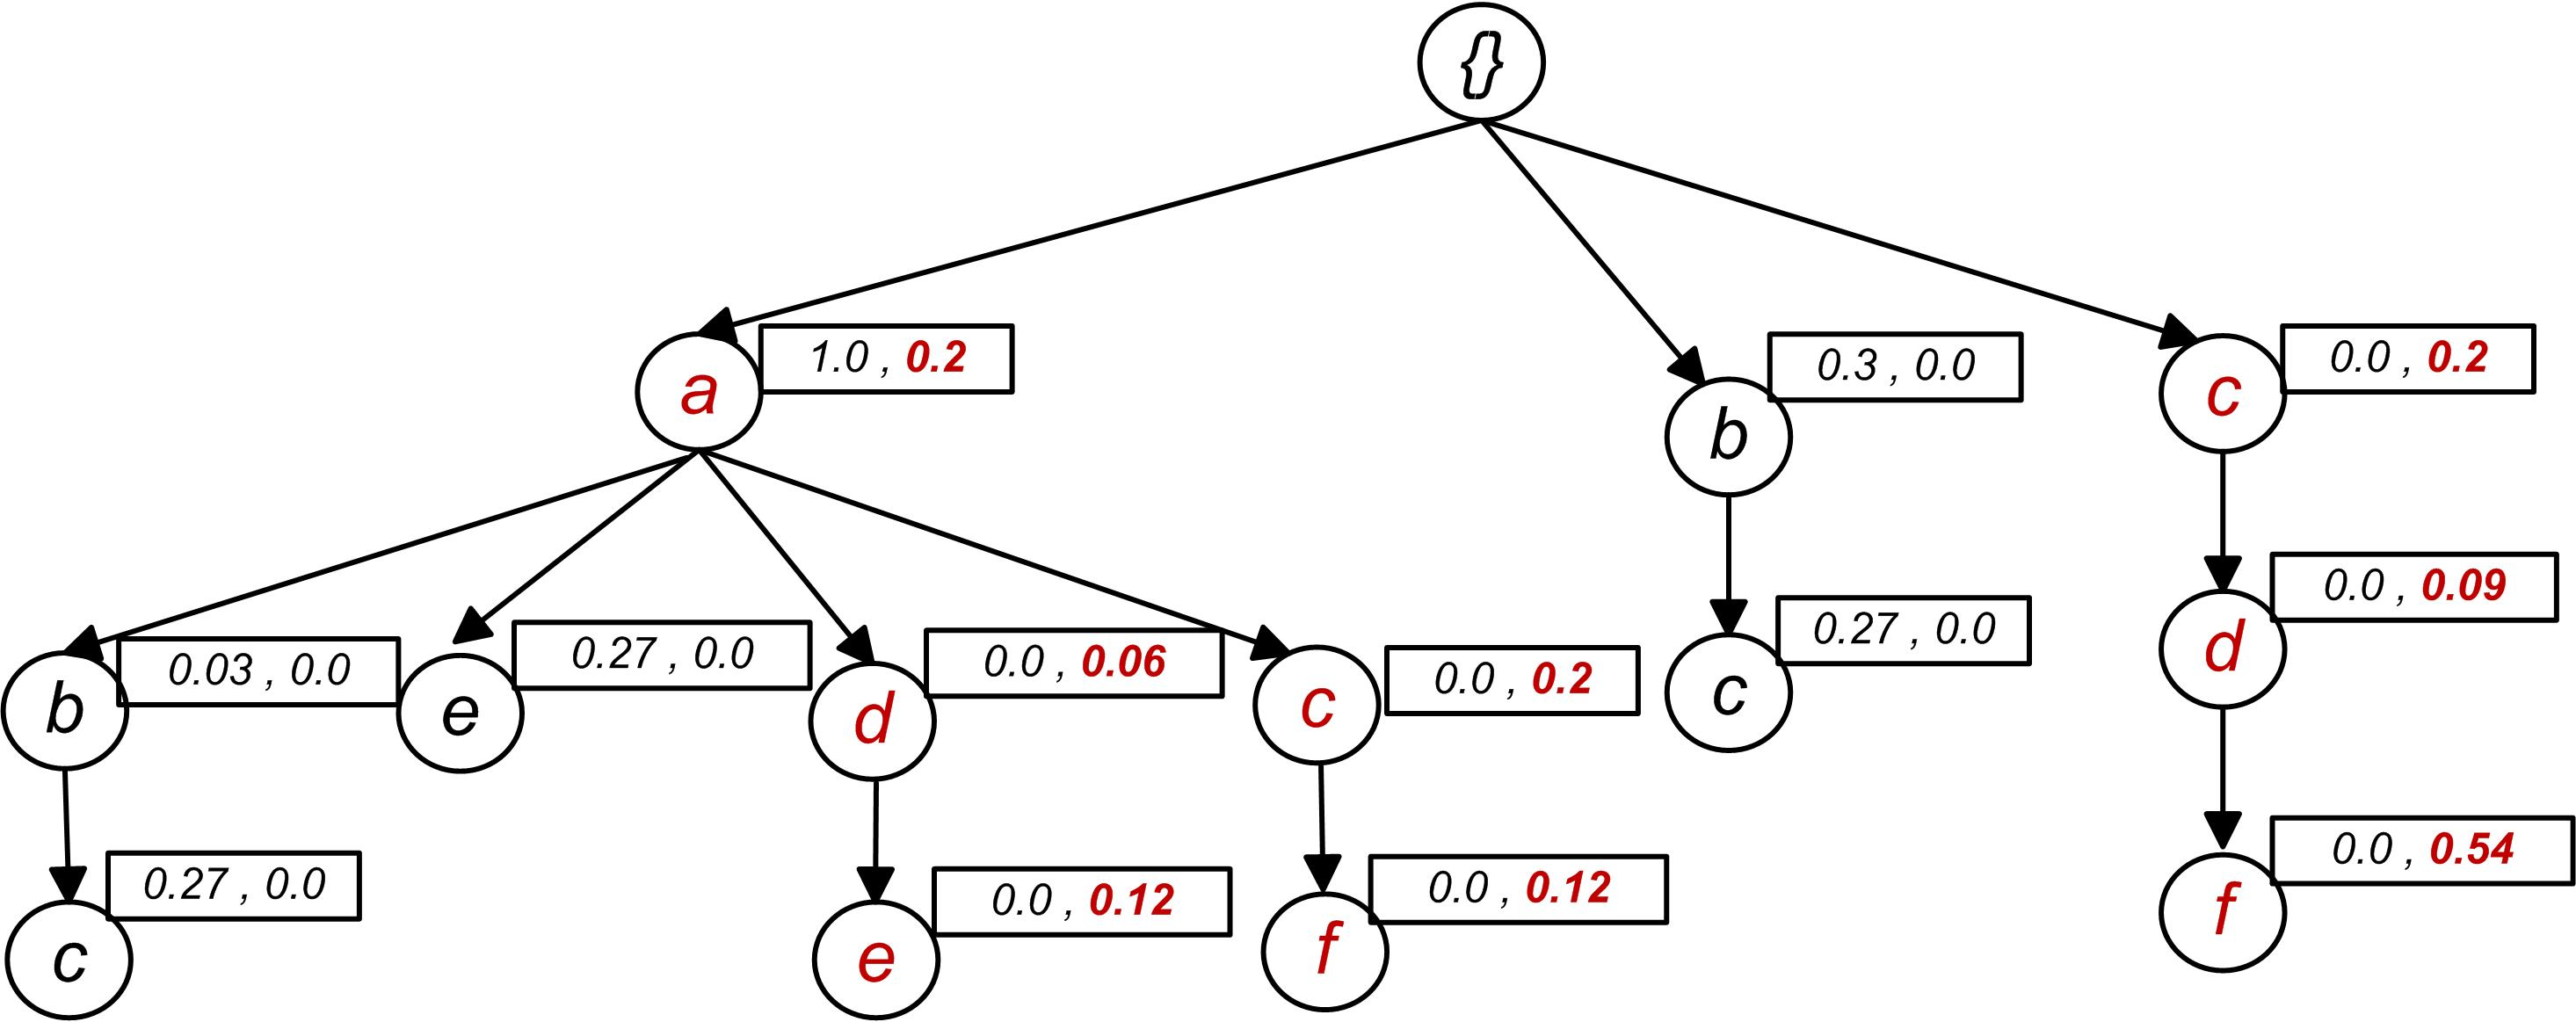
\includegraphics[width=.8\textwidth]{images/sim_789.jpg}  
	\caption{Inserting \emph{T\textsubscript{7}, T\textsubscript{8}, T\textsubscript{9}} into \emph{US-tree} after sliding}
	\label{figure:w2}
\end{figure}
%\end{document}
\subsection*{}
Now our window is completed and can our \emph{USFP-growth} mine \emph {US-tree}. When new transaction batch comes like \emph{Batch-3 (T\textsubscript{7}, T\textsubscript{8}, T\textsubscript{9})} comes to be inserted into the tree then first we have to slide the window. For this when we construct the tree we maintain a header table which contains the information for the oldest data. Thus pointer points to the oldest data can be found easily and slide the whole tree. Figure-\ref{figure:slide} shows the sliding and getting the old data removed tree and ready to insert next batch \emph{Batch-3}. After inserting \emph{Batch-3} we get the tree like Figure-\ref{figure:w2}. 
\documentclass{article}
\usepackage{graphicx}
\usepackage{caption}
\usepackage{subcaption}

\begin{document}

\begin{frame}

\begin{figure}[!tbp]
  \centering
	\fbox{  
	 	\begin{subfigure}[b]{0.44\textwidth}
	 	\centering
	    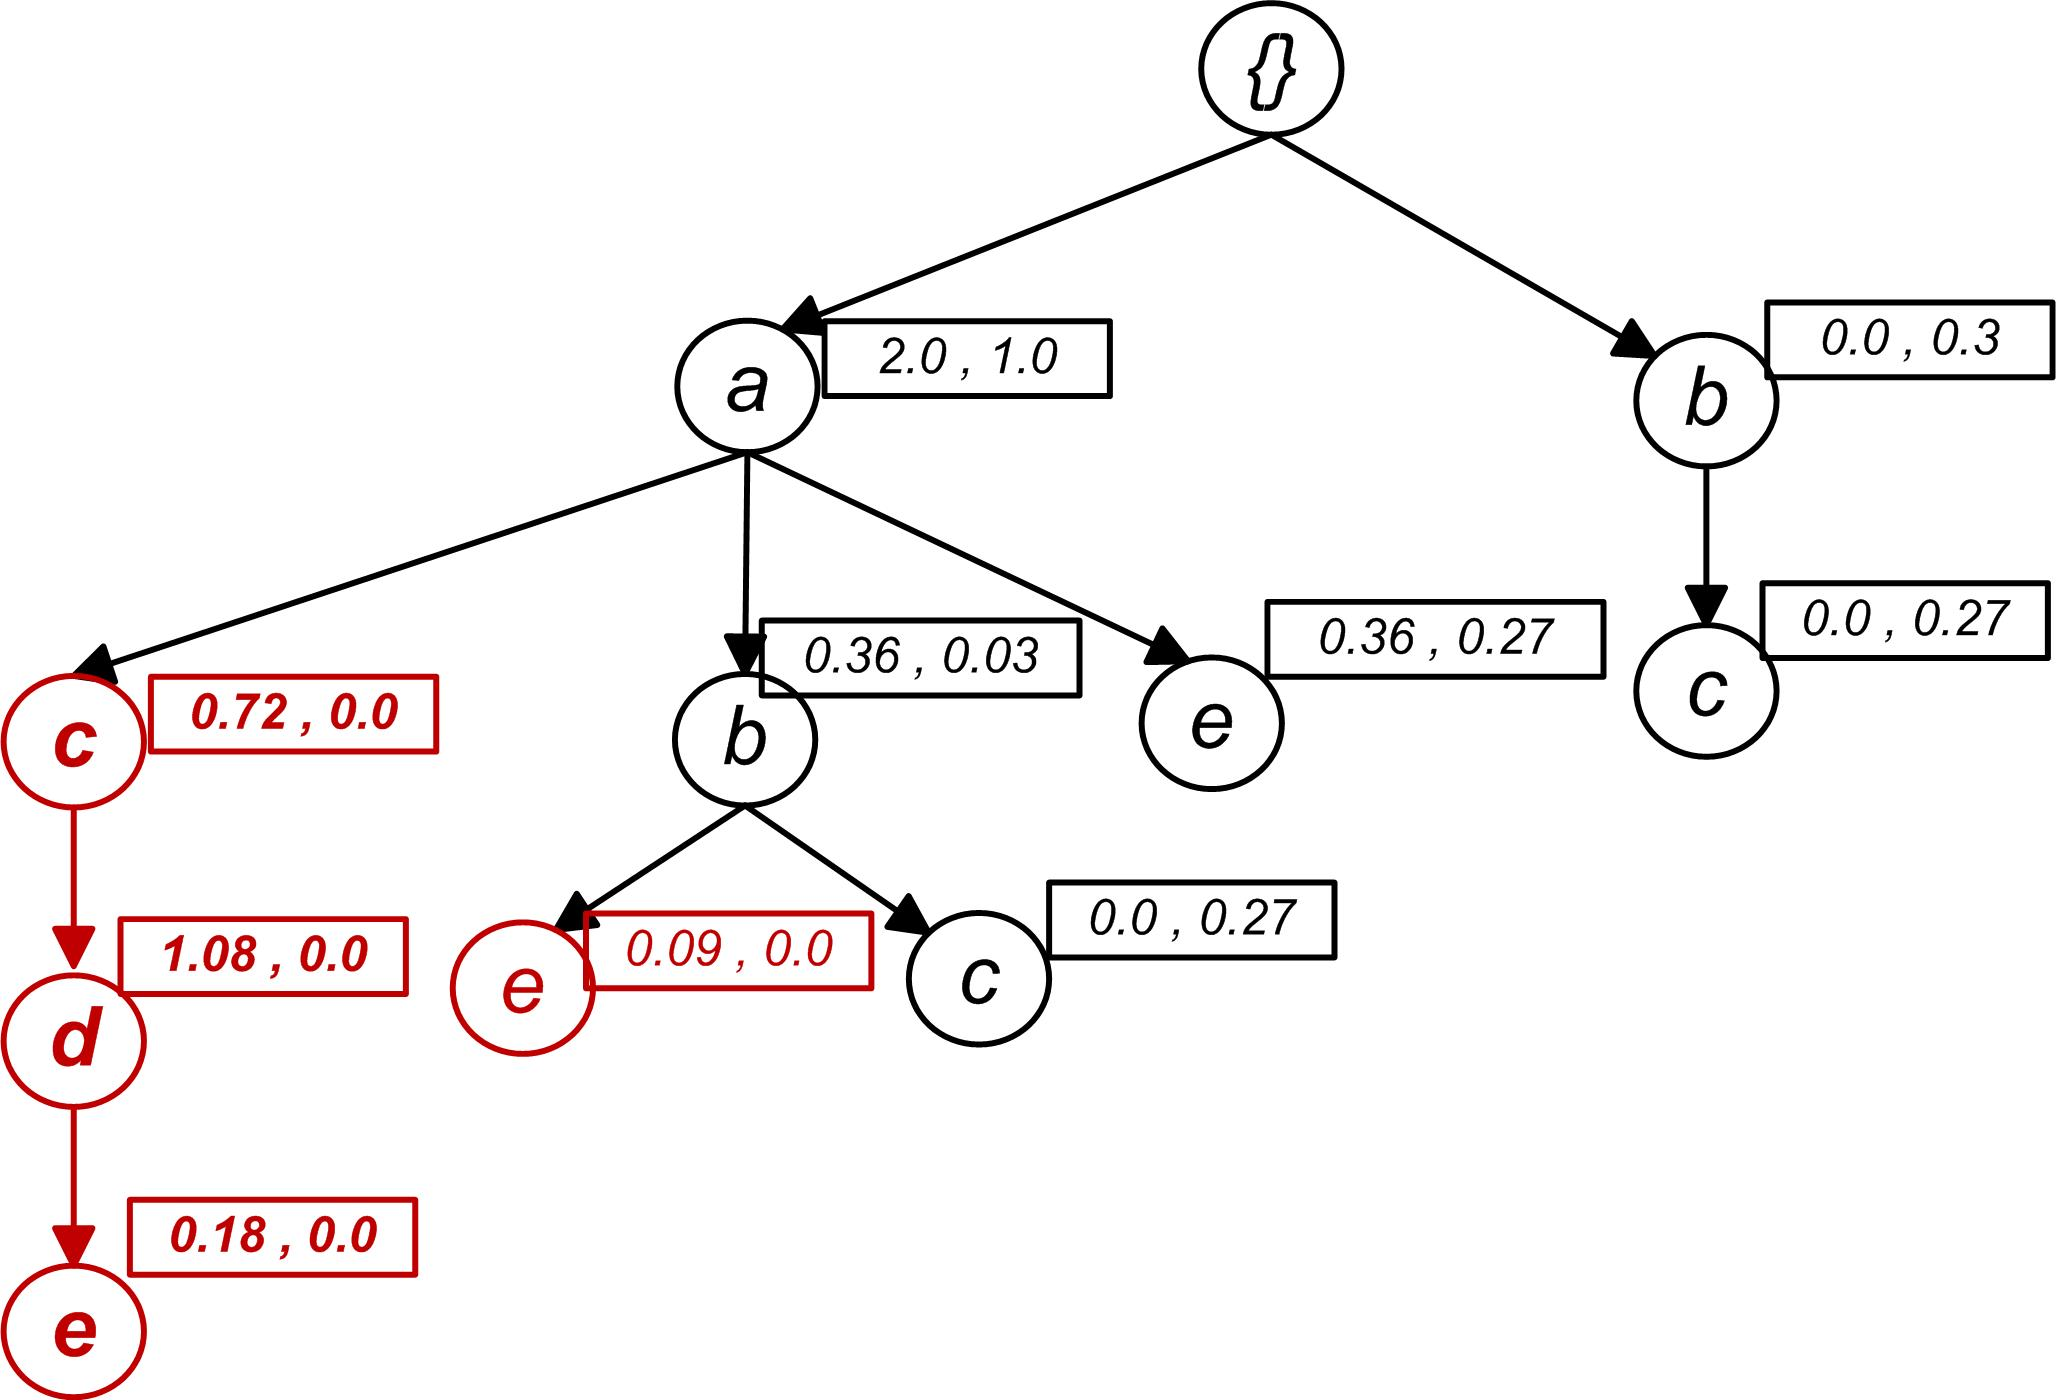
\includegraphics[width=\textwidth,height=4.5cm]{../images/sim_06_slide.jpg}
	    \caption{Before Sliding}
		\end{subfigure}
 
	 	\begin{subfigure}[b]{0.36\textwidth}
	 	\centering
	    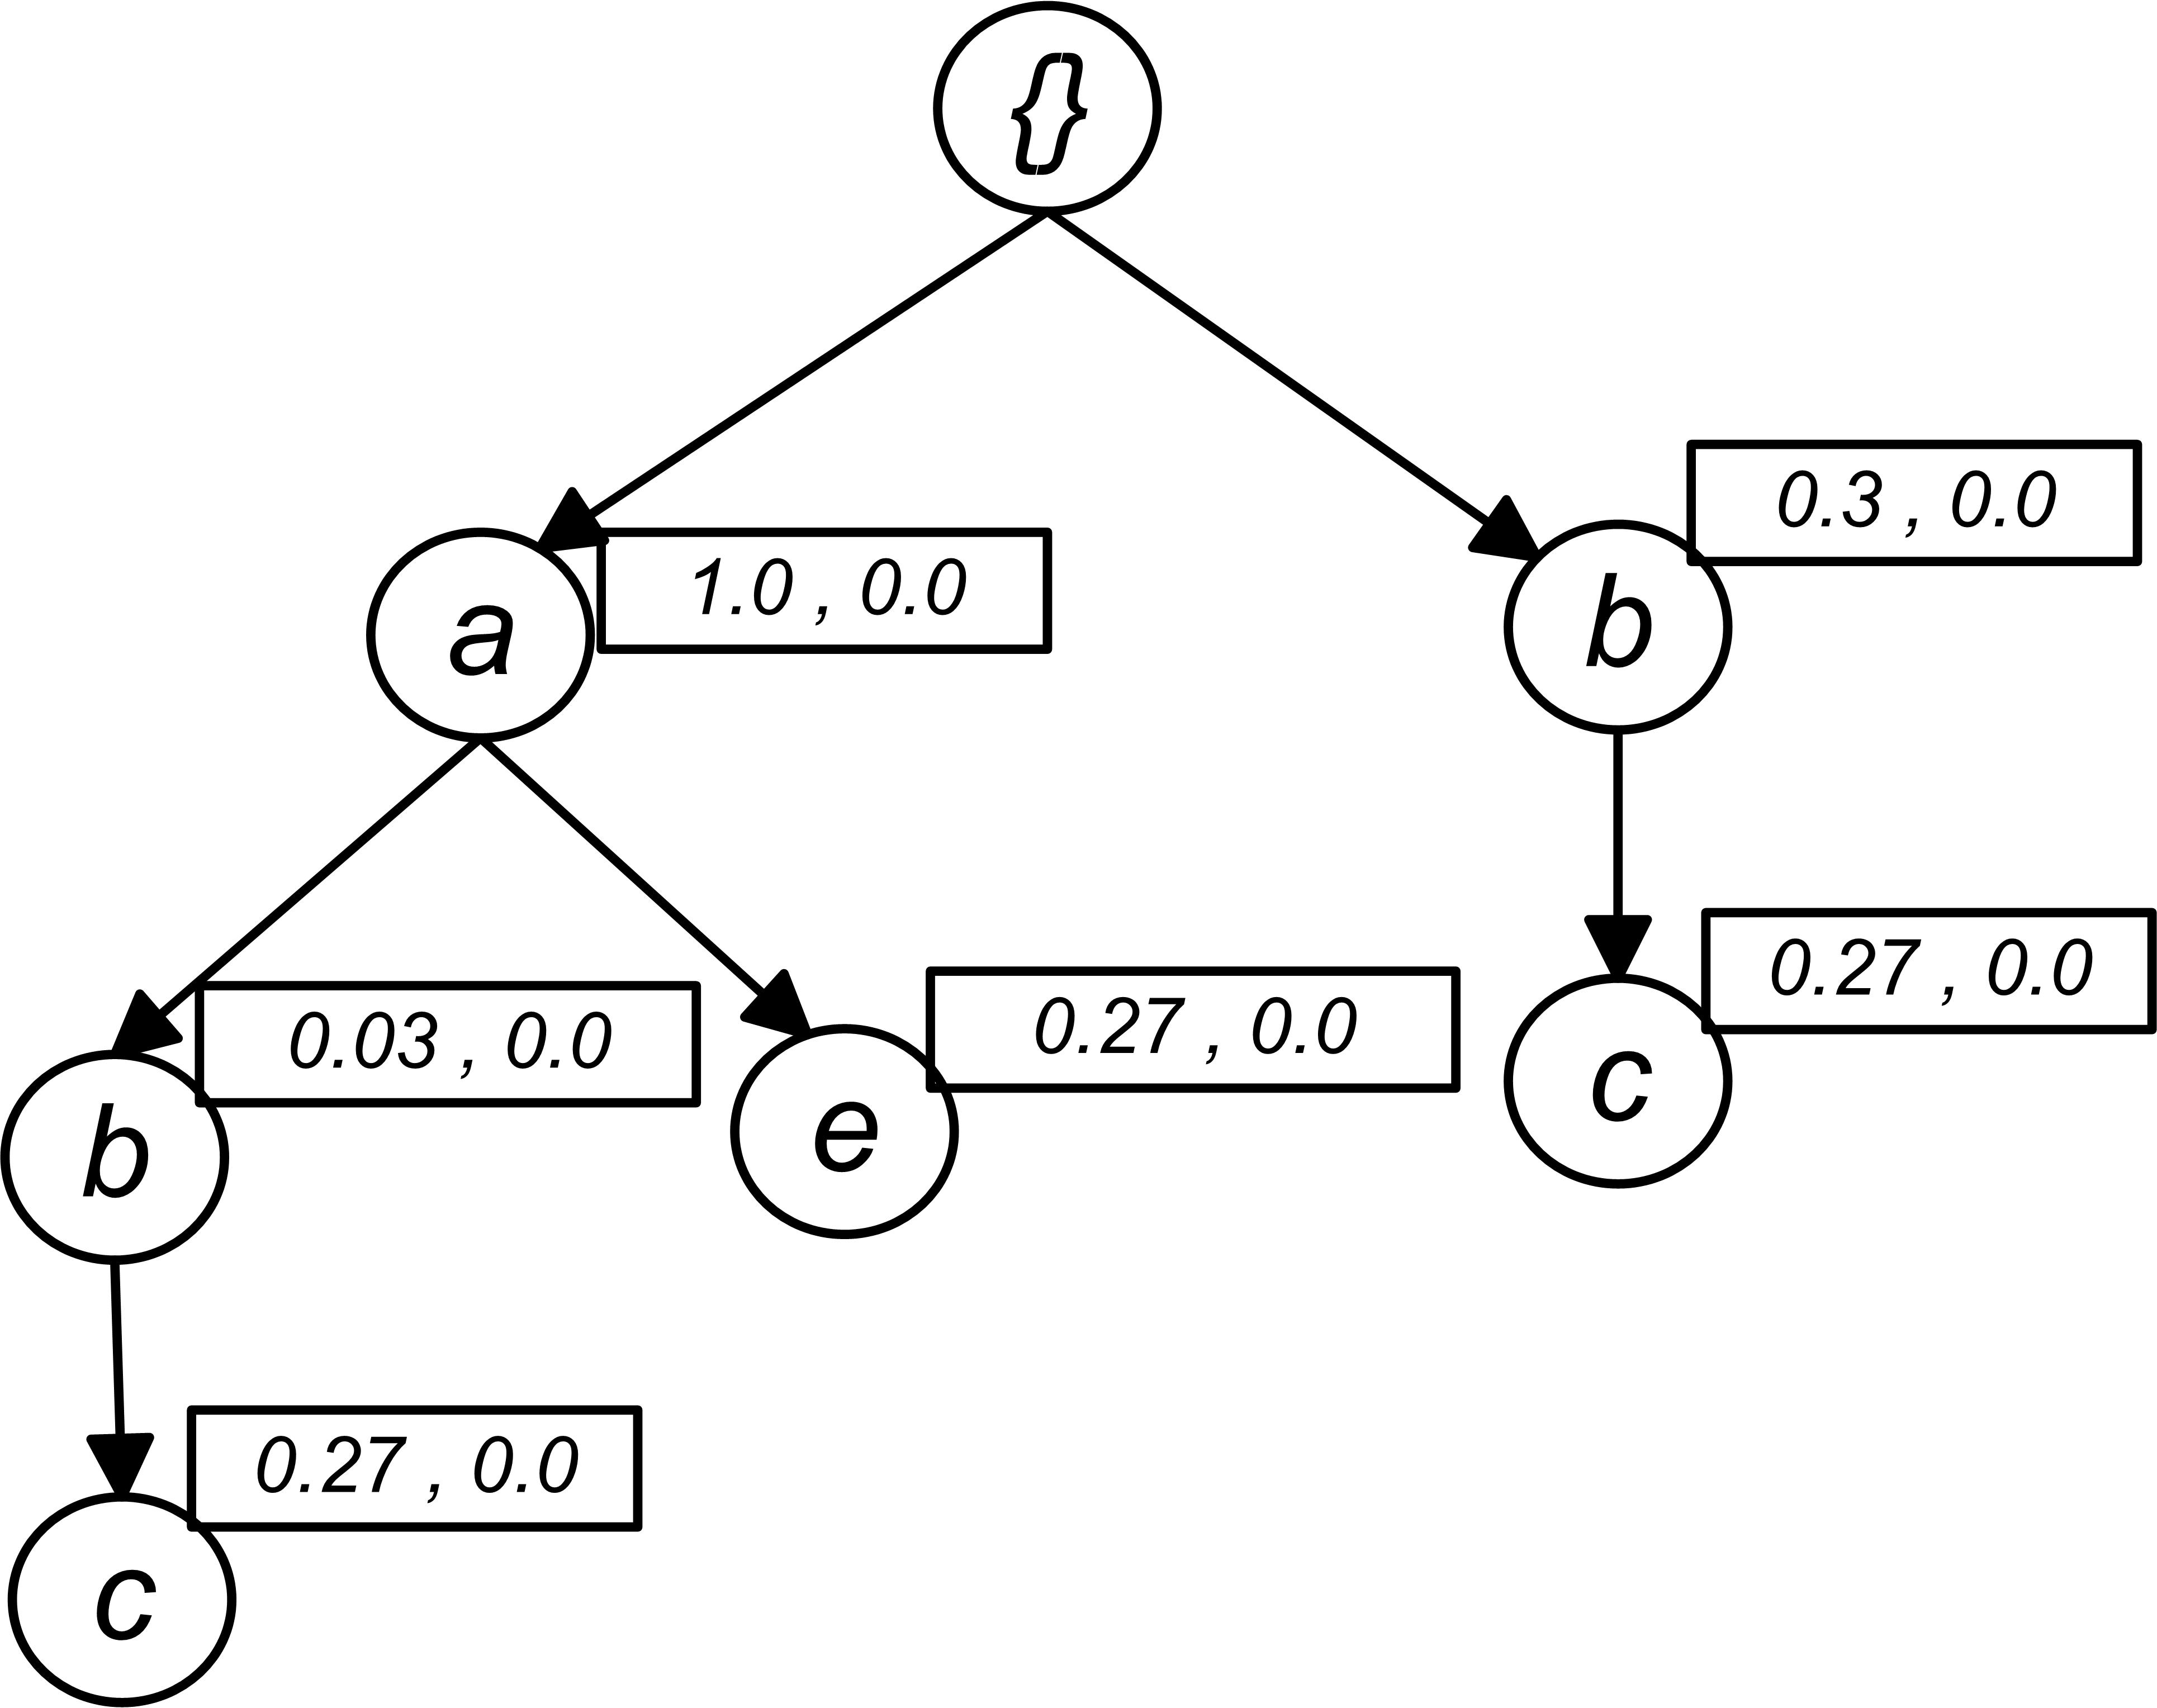
\includegraphics[width=\textwidth,height=4.5cm]{../images/sim_06_slide_2.jpg}
	    \caption{After Sliding}
		\end{subfigure}
	}
 \caption{Sliding \emph{US-tree}}
\end{figure}
\end{frame}



\end{document}
\subsection*{}
In the described \emph{US-tree} construction process we see that tree sharing is very much common and regular. That makes our tree very compact and reduce memory needed to hold the tree. More over the tree construction time improves surprisingly. When to mine this \emph{US-tree} we can gain a lot time when mining. As the tree size is small, conditional tree will be much more less when mining. We will gain a lot time when trying to mine the conditional trees. In the experimental result section we will provide necessary graphs for our simulations.
%\end{document}